%!TEX root=../paper/paper.tex
\section{Evaluation}\label{sec:ccnn_evaluation}

\PM{Dataset}
We evaluate on the standard object detection benchmark: the PASCAL VOC \cite{pascal-voc-2010}.
In all cases, the CNN region classifiers are trained on the PASCAL VOC 2007 trainval set.
The parameters of our methods are set by training or cross-validation on the VOC 2007 val set.
We evaluate on the VOC 2007 test set.
The result plots and details are shown in \autoref{fig:voc2007_results} and \autoref{tab:ccnn_results}.

\PM{Implementation}
The scoring function for the quick-to-compute features is trained by a logistic regression classifier onto the max PASCAL overlap with any ground truth window on the validation dataset.
The classifier is optimized by stochastic gradient descent, and its regularization parameter is cross-validated.
The R-CNN software was used as available in June 2014.
\footnote{\url{https://github.com/rbgirshick/rcnn}}
That software relies on Selective Search \cite{Uijlings-IJCV-2013} region proposals.
Different images are proposed different numbers of regions.
\autoref{fig:roi_hist} shows the distribution of number of regions on the validation set, with the parameters of the R-CNN.
An additional parameter is the size of each batch of regions that goes through the CNN.
We set batch size to 100 regions, and observe that it takes on average 500 ms to process them with the CNN.
In all experiments, we use Ubuntu 12.04, Intel i5 3.2GHz CPU, and NVIDIA Tesla K40 GPU.

%!TEX root=../paper/paper.tex
\begin{figure}[ht]
\begin{subfigure}[b]{\linewidth}
    \centering
    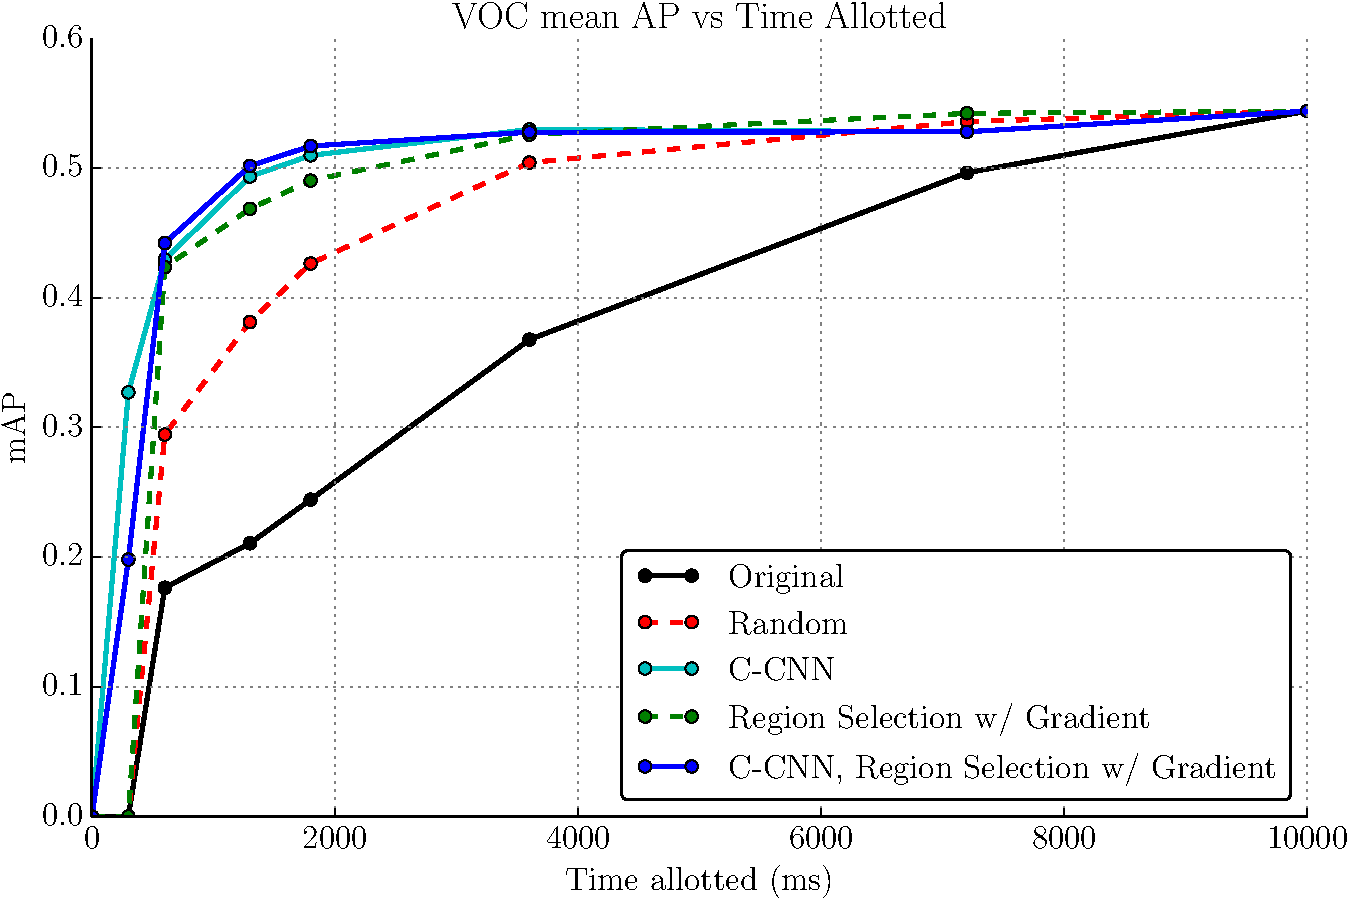
\includegraphics[width=.75\linewidth]{../ccnn/figures/_apvst_final.pdf}
    \caption{
Plotting Mean AP vs. Time Allotted allows comparison performance at a given time budget.
For example, at 1300 ms, random region selection gets about 0.42 mAP, while our best method (C-CNN with gradient-based region selection) obtains 0.50 mAP.
}\label{fig:apvst}
\end{subfigure}
\begin{subfigure}[b]{\linewidth}
    \centering
    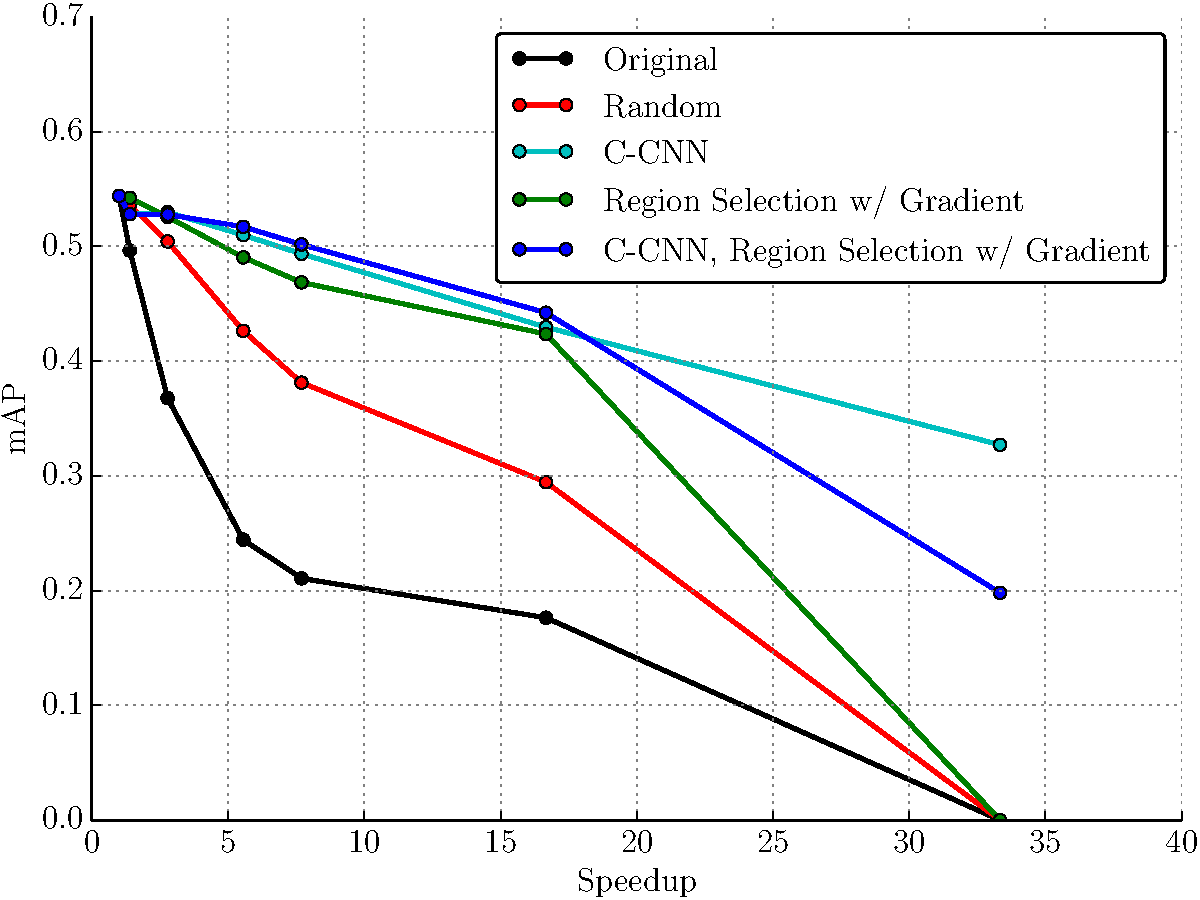
\includegraphics[width=.75\linewidth]{../ccnn/figures/_speedup_final_abs.pdf}
    \caption{
Plotting mean AP vs. speed-up factor allows comparison of speed-ups at a given mAP point.
For example, we can see that we should obtain mAP of 0.40 at around 20x speedup with our method.
}\label{fig:speedup}
\end{subfigure}
\caption{
Results of the Cascade CNN and other Anytime methods on the PASCAL VOC 2007 dataset.
}\label{fig:voc2007_results}
\end{figure}


\begin{table}[ht]
\centering
\caption{
Full table of AP vs. Time results on PASCAL VOC 2007.
Best performance for each time point is in bold.
}\label{tab:results}
\small{
\begin{tabular}{lrrrrrrrr}
\toprule
Time allotted (ms)                  & 0 & 300            & 600            & 1300           & 1800           & 3600           & 7200           & 10000 \\
\midrule
Original                            & 0 & 0.000          & 0.176          & 0.211          & 0.244          & 0.368          & 0.496          & 0.544 \\
Random                              & 0 & 0.000          & 0.295          & 0.381          & 0.426          & 0.504          & 0.536          & 0.544 \\
C-CNN                               & 0 & \textbf{0.327} & 0.430          & 0.493          & 0.510          & 0.528          & 0.528          & - \\
Region Selection w/ Gradient        & 0 & 0.000          & 0.424          & 0.469          & 0.490          & 0.526          & \textbf{0.542} & 0.544 \\
C-CNN, Region Selection w/ Gradient & 0 & 0.198          & \textbf{0.442} & \textbf{0.502} & \textbf{0.517} & \textbf{0.528} & 0.528          & - \\
\bottomrule
\end{tabular}
}
\end{table}


The experimental settings are
\begin{description}
  \item[Original] \hfill \\
  The original order of the Selective Search regions of interest.
  This order is influenced by the hierarchical segmentation of their method, and so has sequences of highly overlapping regions.

  \item[Random] \hfill \\
  A completely blind permutation of the original order.

  \item[Region Selection] \hfill \\
  The region statistics feature is always used.
  Additionally, we consider the Pixel Gradient feature, with \emph{setup time} of the gradient forward-back propagation of 20 ms.

  \item[Cascade CNN] \hfill \\
  The Cascade CNN model, as described in \autoref{sec:ccnn}.
  The first experiment (C-CNN) takes batches of regions in a random order.
  The next two experiments also make use of the Region Selection methodology with the quick-to-compute feature.
\end{description}

\PM{Analysis}
Since the time to process a full batch with a non-Cascade CNN is 500 ms, there are no results for non-cascaded baselines at 300 ms.
At this time, the Cascade CNN without any region ordering is best.
A reason for why C-CNN with Region Selection is not as good at this point is that the region selection presents better region candidates, with fewer rejection opportunities, and thus has less coverage of the image.
At 600 ms, C-CNN method have had more than one batch go through, and the Region Selection is giving it a lead over the simple C-CNN.
Both method are better than the baseline non-cascaded methods for this entire duration.
